\section{Throughput}
In this section, we'll estimate the throughput of MultiPaxos, EPaxos, and
Simple BPaxos. We'll show that under some simplifying assumptions, Simple
BPaxos achieves higher throughput than the other two protocols. We'll then
discuss how these simplifying assumptions are not exactly true.

\subsection{MultiPaxos Throughput}
Let's begin by reviewing MultiPaxos. MultiPaxos is composed of an arbitrary
number of clients, a set of $p$ proposers (where $l \geq f + 1$), and a set of
$n = 2f + 1$ acceptors. We assume that one of the proposers is elected as a
stable leader.  We further assume that proposers double as replicas (i.e., each
proposer manages a replica of the state machine).

To get a command executed, a client sends the command to the leader, the leader
sends phase 2a messages to the acceptors, the acceptors respond with phase 2b
messages, the leader executes the command, the leader informs the other
proposers that the command has been chosen, and the leader sends back a reply
to the client. This is illustrated in \figref{multipaxos}.

\begin{figure}[ht]
  \centering
  \tikzstyle{proc}=[draw, thick, circle, inner sep=3pt]
  \tikzstyle{msg}=[-latex, thick]
  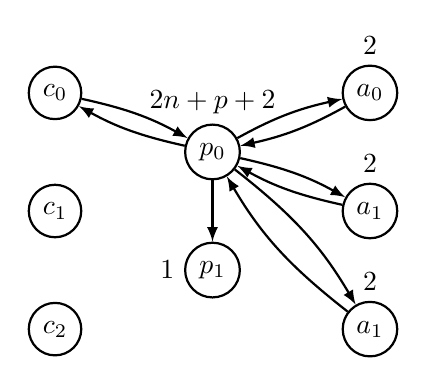
\begin{tikzpicture}[xscale=2, yscale=1.5]
    \node[proc] (client1) at (0, 2) {$c_0$};
    \node[proc] (client2) at (0, 1) {$c_1$};
    \node[proc] (client3) at (0, 0) {$c_2$};
    \node[proc, label=$2n+p+2$] (proposer1) at (1, 1.5) {$p_0$};
    \node[proc, label={180:$1$}] (proposer2) at (1, 0.5) {$p_1$};
    \node[proc, label=$2$] (acceptor1) at (2, 2) {$a_0$};
    \node[proc, label=$2$] (acceptor2) at (2, 1) {$a_1$};
    \node[proc, label=$2$] (acceptor3) at (2, 0) {$a_1$};
    \draw[msg, bend left=10] (client1) to (proposer1);
    \draw[msg, bend left=10] (proposer1) to (acceptor1);
    \draw[msg, bend left=10] (proposer1) to (acceptor2);
    \draw[msg, bend left=10] (proposer1) to (acceptor3);
    \draw[msg, bend left=10] (acceptor1) to (proposer1);
    \draw[msg, bend left=10] (acceptor2) to (proposer1);
    \draw[msg, bend left=10] (acceptor3) to (proposer1);
    \draw[msg] (proposer1) to (proposer2);
    \draw[msg, bend left=10] (proposer1) to (client1);
  \end{tikzpicture}
  \caption{MultiPaxos}\figlabel{multipaxos}
\end{figure}

We want to estimate the peak throughput of MultiPaxos. To do so, we'll estimate
roughly how much time each participant takes to process a single command. The
participant that requires the most amount of time is the bottleneck and
dictates the throughput of the protocol. For example, if a proposer spends
$0.5$ seconds on each command, and an acceptor spends $0.1$ second on each
command, then the proposer is the bottleneck and MultiPaxos can process at most
two commands per second.

To estimate how long each participant takes to process a command, we'll make
the \emph{critical simplifying assumption} that the time taken is directly
proportional to the number of messages processed (either sent or received).
For example, in \figref{multipaxos}, the leader processes a total of $2n + p +
2$ messages ($n + 1$ received, $n + p + 2$ sent), the other proposers process
one message, and every acceptor processes a total of two messages (one sent,
one received). Thus, the leader requires time proportional to $2n + p + 2$
while the proposers and acceptors require time proportional to $1$ and $2$
respectively. $2n + p + 2$ is larger than $1$ and $2$, so the leader is the
bottleneck, and the throughput of MultiPaxos is proportional to $(2n + p +
2)^{-1}$.

Can we eliminate this bottleneck by adding more leaders? No. MultiPaxos
requires a single leader for good performance. With multiple leaders, you run
into the dueling leaders problem and performance collapses.

\subsection{EPaxos Throughput}
Next, we estimate the throughput of EPaxos. EPaxos is composed of a number of
clients and a set of $n = 2f + 1$ replicas. To get a command executed on the
fast path, a client sends the command to a replica, the replica sends PreAccept
messages to the other replicas, the other replicas respond with PreAcceptOk
messages, the replica executes the command, the replica informs the other
replicas that the command has been chosen, and the replica responds to the
client. It's also possible that EPaxos takes the slow path, but we'll be
optimistic and assume the fast path is always taken.

\begin{figure}[ht]
  \centering
  \tikzstyle{proc}=[draw, thick, circle, inner sep=3pt]
  \tikzstyle{msg}=[-latex, thick]
  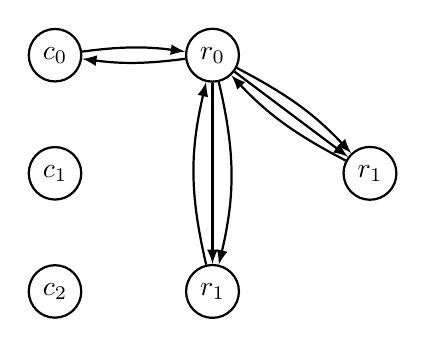
\begin{tikzpicture}[xscale=2, yscale=1.5]
    \node[proc] (client1) at (0, 2) {$c_0$};
    \node[proc] (client2) at (0, 1) {$c_1$};
    \node[proc] (client3) at (0, 0) {$c_2$};
    \node[proc] (replica1) at (1, 2) {$r_0$};
    \node[proc] (replica2) at (2, 1) {$r_1$};
    \node[proc] (replica3) at (1, 0) {$r_1$};
    \draw[msg, bend left=10] (client1) to (replica1);
    \draw[msg, bend left=10] (replica1) to (replica2);
    \draw[msg, bend left=10] (replica1) to (replica3);
    \draw[msg, bend left=10] (replica2) to (replica1);
    \draw[msg, bend left=10] (replica3) to (replica1);
    \draw[msg] (replica1) to (replica2);
    \draw[msg] (replica1) to (replica3);
    \draw[msg, bend left=10] (replica1) to (client1);
  \end{tikzpicture}
  \caption{EPaxos}\figlabel{epaxos}
\end{figure}


This is illustrated in \figref{epaxos}. We see that the leader replica
processes $1 + 2(n-1) + (n-1) + 1 = 3n - 1$ messages for every command. Thus,
the maximum throughput of the leader replica is proportional to $(3n -
1)^{-1}$. Actually, it's a little bit lower than that because the replica has
to process messages from the other replicas, but we'll ignore this detail.
Every EPaxos replica can concurrently process messages, so the peak throughput
of the protocol is proportional to $n(3n-1)^{-1}$.

Can we increase the throughput of the protocol by increasing $f$? No. $3n - 1$
is larger than $n$, so increasing $n$ actually reduces the throughput. We can
implement thriftiness and batch the messages sent from one replica to another,
but the throughput will always decrease with more replicas.

\subsection{Simple BPaxos Throughput}
Simple BPaxos is composed of a number of clients, $l$ leaders and proposers, $n
= 2f+1$ dependency service nodes, $n$ acceptors, and $f + 1$ replicas. To get a
command executed, a client sends the command to a leader, the leader sends
dependency request messages to the dependency service nodes, the dependency
service nodes respond with dependencies, the leader takes the union of the
dependencies and forwards them to a co-located proposer, the proposer sends
phase 2a messages to the acceptors, the acceptors send back phase 2b messages,
the proposer forwards the chosen command to all the replicas, all replicas
execute the command, and one of the replicas sends the reply back to the
client. This is illustrated in \figref{simplebpaxos}.

\begin{figure}[ht]
  \centering
  \tikzstyle{proc}=[draw, thick, circle, inner sep=3pt]
  \tikzstyle{msg}=[-latex, thick]
  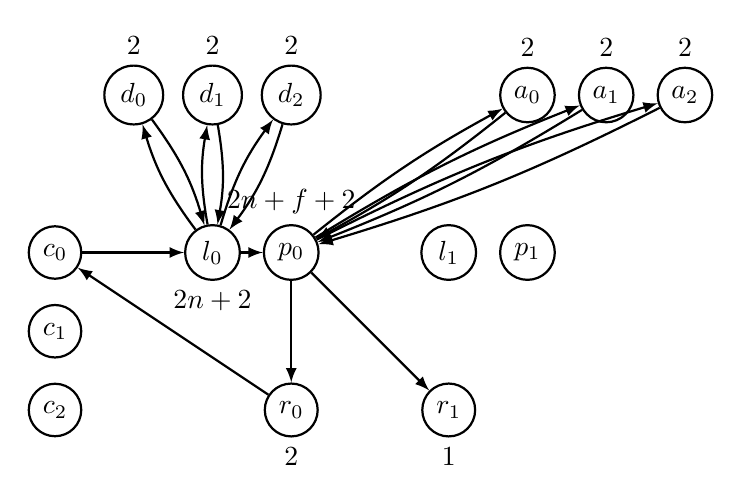
\begin{tikzpicture}[xscale=1, yscale=1]
    \node[proc] (client0) at (0, 2) {$c_0$};
    \node[proc] (client1) at (0, 1) {$c_1$};
    \node[proc] (client2) at (0, 0) {$c_2$};
    \node[proc, label={270:$2n+2$}] (leader0) at (2, 2) {$l_0$};
    \node[proc] (leader1) at (5, 2) {$l_1$};
    \node[proc, label={90:$2n+f+2$}] (proposer0) at (3, 2) {$p_0$};
    \node[proc] (proposer1) at (6, 2) {$p_1$};
    \node[proc, label={90:$2$}] (dep0) at (1, 4) {$d_0$};
    \node[proc, label={90:$2$}] (dep1) at (2, 4) {$d_1$};
    \node[proc, label={90:$2$}] (dep2) at (3, 4) {$d_2$};
    \node[proc, label={90:$2$}] (acceptor0) at (6, 4) {$a_0$};
    \node[proc, label={90:$2$}] (acceptor1) at (7, 4) {$a_1$};
    \node[proc, label={90:$2$}] (acceptor2) at (8, 4) {$a_2$};
    \node[proc, label={270:$2$}] (replica0) at (3, 0) {$r_0$};
    \node[proc, label={270:$1$}] (replica1) at (5, 0) {$r_1$};
    \draw[msg] (client0) to (leader0);
    \draw[msg, bend left=10] (leader0) to (dep0);
    \draw[msg, bend left=10] (leader0) to (dep1);
    \draw[msg, bend left=10] (leader0) to (dep2);
    \draw[msg, bend left=10] (dep0) to (leader0);
    \draw[msg, bend left=10] (dep1) to (leader0);
    \draw[msg, bend left=10] (dep2) to (leader0);
    \draw[msg] (leader0) to (proposer0);
    \draw[msg, bend left=5] (proposer0) to (acceptor0);
    \draw[msg, bend left=5] (proposer0) to (acceptor1);
    \draw[msg, bend left=5] (proposer0) to (acceptor2);
    \draw[msg, bend left=5] (acceptor0) to (proposer0);
    \draw[msg, bend left=5] (acceptor1) to (proposer0);
    \draw[msg, bend left=5] (acceptor2) to (proposer0);
    \draw[msg] (proposer0) to (replica0);
    \draw[msg] (proposer0) to (replica1);
    \draw[msg] (replica0) to (client0);
  \end{tikzpicture}
  \caption{Simple BPaxos}\figlabel{simplebpaxos}
\end{figure}

The dependency service nodes and acceptors all process two messages. The
replicas process either one or two messages. The leaders and proposers process
$2n+2$ and $2n + f + 2$ messages. Thus, the proposers are the bottleneck. The
dependency service, acceptors, and replicas can achieve a peak throughput
proportional to $\frac{1}{2}$, while the proposers are bottlenecked at a peak
throughput proportional to $l(2n+f+2)^{-1}$.

Can we eliminate this bottleneck by increasing the number of leaders and
proposers? Yes! Leaders and proposers do not interact with one another, so we
can increase the number of leaders and proposers without increasing the number
of messages they have to handle. If we increase $l$ enough, the leaders and
proposers stop being the bottleneck, and the protocol instead becomes
bottlenecked by the dependency service, acceptors, and replicas. Moreover, the
dependency service, acceptors, and replicas are only processing two messages
per command! It's hard to do better than that.

In summary, MultiPaxos is fundamentally bottlenecked by a single leader. EPaxos
colocates every participant, so the number of leaders is fixed at $2f + 1$.
This prevents EPaxos from scaling the number of leaders and proposers without
scaling $f$, and scaling $f$ decreases peak throughput. Simple BPaxos decouples
all the participants of the protocol. This decoupling seems inconsequential,
but it actually allows us to easily scale up the bottleneck participants and
get a protocol with very good peak throughput. Moreover, this idea is not
limited to Simple BPaxos. We can apply the same idea to Unanimous BPaxos or
Majority Commit BPaxos and get a protocol with higher throughput than EPaxos
with similar or better latency.

In fact, we can apply the same idea to other protocols like Mencius. Mencius
also colocates leaders with acceptors, limiting the number of leaders to $n$.
If we decouple leaders from acceptors, we can scale up the leaders until they
are no longer the bottleneck and achieve throughput that should be identical to
Simple BPaxos. I haven't fully vetted this idea though, so it could be wrong.
The latency of the protocol will also likely suffer.

% TODO(mwhittaker): More aggressive BPaxos scaling.
% TODO(mwhittaker): Section on Mencius.
% TODO(mwhittaker): Section on SPaxos.
% TODO(mwhittaker): Section on NoPaxos?

\subsection{Faulty Assumptions}
Up to now, we've made the fundamental assumption that the time required to
process a command is directly proportional to the number of messages processed
for the command. Unfortunately, this is not true in practice. Empirically, we
find that Simple BPaxos replicas quickly become a bottleneck. Every replica has
to reverse topologically sort the strongly connected components of a graph.
This can become a bottleneck, even though the replicas are not processing many
messages. Thus far, I've implemented an efficient algorithm to do this and have
performed batching to speed things up more, but it still seems like it's a
bottleneck. More work has to be done to see if we can eliminate the bottleneck.

\subsection{Colocation and Thriftiness}
MultiPaxos and EPaxos can both benefit from thriftiness and colocation.
Colocating the MultiPaxos leader with one of the acceptors and implementing
thriftiness, the time required per command is proportional to $1 + 2f + (p-1) +
1 = n + p$, and the peak thriftiness is proportional to $(n + p)^{-1}$.

When EPaxos replicas implement thriftiness, the time required per command is
proportional to
\[
  1 + 2 (f + \floor{(f+1)/2} - 1) + n-1 + 1
  = 2n + f - 1
\]
If we do not ignore the cross-replica communication, then for every set of $n$
commands sent to $n$ replicas, every replica has to process roughly $3(n-1) +
(n-1)$ extra commands (this ignores thriftiness). So, the time on a single
replica for a batch of $n$ commands is proportional to $5n + f - 4$, and the
peak throughput is proportional to $n(5n + f - 4)^{-1}$.
